% !TeX root = ./AER Insights.tex
% Last updated:
% 6 Aug 18- CC


% EXHIBIT: PRODUCTIVITY TABLE
% \clearpage

% !TeX root = ../AER Insights.tex
%tab_prodfcn_2008_old.tex
%Ian M. Schmutte
% 2018-10-29
% Uses results from C:\Users\schmutte\Dropbox\MGMT_source\output\IBGE\tables\ly_collapse.tex

\begin{table}[h t]
  \caption{Production Function Estimates: WMS-RAIS-PIA Matched Data} \label{tab:e1_prodfcn}
  \begin{center}
\begin{tabular}{lcccccc}
    \toprule
\textbf{Dependent variable: ln(sales)}                                  	& (1)      & (2)       & (3)       & (4)     & (5) & (6)  \\
    \midrule\
\textbf{Management score} \\
z-management                  &0.213*** & 0.168*** & 0.088*** & 0.065***& 0.064***& 0.059***  	\\
                                  	&(0.039) 	& (0.039) 	& (0.02)   	& (0.01)    & (0.01)    & (0.01)    		\\
\textbf{AKM quality measures} \\
z-worker quality           &	  	& 0.247***	& 0.076*** &           	&           	&           		\\
                                  	&	  	& (0.039)   	& (0.02)     &           	&          	& 			\\
~ ~ z-production worker quality   &       	&          	& 		& 0.031**  & 0.028*   & 0.010     	\\
                                  	&	 	&          	& 		& (0.02)    & (0.02)    & (0.02)    		\\
~ ~ z-manager quality       &       	&          	& 		& 0.078*** & 0.076***& 0.053***  	\\
                                  	& 		& 		&          	& (0.02)    	& (0.02)    	& (0.02)    \\
z-firm quality               	&          	&           	&           	&		&		& 0.098***  \\
                                  	&          	&           	&           	& 		&		& (0.02)    \\	
\textbf{Firm characteristics} \\
Share workers with college degree & &           	& 		& 		& 0.05      	& 0.05      \\
                                  	& 		&          	& 		& 		& (0.10)    & (0.10)    \\
\midrule
Factor inputs	 		& 		& 	 	& Y 		& 	Y 	& 	Y	& Y \\
Industry				& Y 		& 	Y 	& Y 		& 	Y 	& 	Y	& Y \\
Ownership			& Y 		& 	Y 	& Y 		& 	Y 	& 	Y	& Y \\
\# Observations              	& 775 	& 775 	& 773      & 663       & 663       & 663    \\
\# Firms                          	& 679 	& 679 	& 679      & 594       & 594       & 594    \\
$R^2 $                            	& 0.753 	& 0.796 	& 0.96     & 0.97      & 0.97      & 0.97      \\
\bottomrule
\end{tabular}
\end{center}
\footnotesize{Notes: Results from OLS regressions of log sales onto the variables described. In addition to the
reported variables, the estimated models also include: industry dummies, and the log of capital, raw materials, and the number of employees. The data are prepared by merging the WMS, RAIS, and PIA samples for years 2008 and 2013.
  }
\end{table}


% \begin{table}
% 	\caption{Correlates of Production Worker and Manager Quality} \label{tab:zpe_mgmt}
% 	\scalebox{0.8}{
% 		\singlespace
% 		\small
% 			\subcaption{PANEL A: TITLE HERE}
% 			
\begin{tabular}{l*{6}{c}}
\toprule
                &\multicolumn{1}{c}{(1)}&\multicolumn{1}{c}{(2)}&\multicolumn{1}{c}{(3)}&\multicolumn{1}{c}{(4)}&\multicolumn{1}{c}{(5)}&\multicolumn{1}{c}{(6)}\\
                &\multicolumn{1}{c}{\textcolor{black}{Avg.\ wrkr FE}}&\multicolumn{1}{c}{\textcolor{black}{Avg.\ wrkr FE}}&\multicolumn{1}{c}{\textcolor{black}{Avg.\ mngr FE}}&\multicolumn{1}{c}{\textcolor{black}{Avg.\ mngr FE}}&\multicolumn{1}{c}{\textcolor{black}{Avg. prod.\ FE}}&\multicolumn{1}{c}{\textcolor{black}{Avg. prod.\ FE}}\\
\midrule
z-operations    &    0.131***&    0.034   &    0.252***&    0.137***&    0.090** &    0.004   \\
                &  (0.042)   &  (0.040)   &  (0.041)   &  (0.040)   &  (0.044)   &  (0.043)   \\
z-people        &    0.079*  &    0.091** &   -0.005   &    0.007   &    0.085*  &    0.098** \\
                &  (0.040)   &  (0.038)   &  (0.037)   &  (0.035)   &  (0.044)   &  (0.042)   \\
Firm controls   &       No   &      Yes   &       No   &      Yes   &       No   &      Yes   \\
Industry controls &      Yes   &      Yes   &      Yes   &      Yes   &      Yes   &      Yes   \\
\midrule
\# Observations &\multicolumn{1}{c}{955}   &\multicolumn{1}{c}{955}   &\multicolumn{1}{c}{955}   &\multicolumn{1}{c}{955}   &\multicolumn{1}{c}{955}   &\multicolumn{1}{c}{955}   \\
\# Firms        &      690   &      690   &      690   &      690   &      690   &      690   \\
\(R^{2}\)       &    0.249   &    0.324   &    0.267   &    0.360   &    0.217   &    0.273   \\
\bottomrule
\end{tabular}

% 			\\ ~
% 			\subcaption{PANEL B: TITLE HERE}
% 			
\begin{tabular}{l*{6}{c}}
\toprule
                &\multicolumn{1}{c}{(1)}&\multicolumn{1}{c}{(2)}&\multicolumn{1}{c}{(3)}&\multicolumn{1}{c}{(4)}&\multicolumn{1}{c}{(5)}&\multicolumn{1}{c}{(6)}\\
                &\multicolumn{1}{c}{\textcolor{black}{Avg.\ wrkr FE}}&\multicolumn{1}{c}{\textcolor{black}{Avg.\ wrkr FE}}&\multicolumn{1}{c}{\textcolor{black}{Avg.\ mngr FE}}&\multicolumn{1}{c}{\textcolor{black}{Avg.\ mngr FE}}&\multicolumn{1}{c}{\textcolor{black}{Avg. prod.\ FE}}&\multicolumn{1}{c}{\textcolor{black}{Avg. prod.\ FE}}\\
\midrule
z-talent mindset        &    0.071** &    0.086***&    0.040   &    0.059*  &    0.078** &    0.091** \\
                &  (0.035)   &  (0.033)   &  (0.035)   &  (0.031)   &  (0.038)   &  (0.036)   \\
z-performance culture        &    0.053   &    0.022   &    0.045   &    0.008   &    0.042   &    0.016   \\
                &  (0.033)   &  (0.032)   &  (0.034)   &  (0.032)   &  (0.034)   &  (0.033)   \\
z-talent capacity        &   -0.024   &   -0.014   &   -0.029   &   -0.018   &   -0.037   &   -0.027   \\
                &  (0.032)   &  (0.031)   &  (0.034)   &  (0.032)   &  (0.033)   &  (0.033)   \\
z-talent development        &   -0.002   &    0.018   &   -0.031   &   -0.013   &    0.012   &    0.032   \\
                &  (0.039)   &  (0.037)   &  (0.038)   &  (0.035)   &  (0.043)   &  (0.041)   \\
z-value proposition        &    0.049   &    0.018   &    0.019   &   -0.015   &    0.043   &    0.016   \\
                &  (0.036)   &  (0.034)   &  (0.041)   &  (0.037)   &  (0.037)   &  (0.036)   \\
Retaining Talent        &   -0.021   &    0.007   &   -0.040   &   -0.009   &   -0.007   &    0.017   \\
                &  (0.036)   &  (0.036)   &  (0.033)   &  (0.033)   &  (0.038)   &  (0.038)   \\
Firm controls   &       No   &      Yes   &       No   &      Yes   &       No   &      Yes   \\
Industry controls &      Yes   &      Yes   &      Yes   &      Yes   &      Yes   &      Yes   \\
\midrule
\# Observations &\multicolumn{1}{c}{955}   &\multicolumn{1}{c}{955}   &\multicolumn{1}{c}{955}   &\multicolumn{1}{c}{955}   &\multicolumn{1}{c}{955}   &\multicolumn{1}{c}{955}   \\
\# Firms        &      690   &      690   &      690   &      690   &      690   &      690   \\
\(R^{2}\)       &    0.255   &    0.327   &    0.272   &    0.362   &    0.223   &    0.277   \\
\bottomrule
\end{tabular}

% "MGMT: Instilling a Talent Mindset"
% "MGMT: Building a High-Performance Culture" 
% "MGMT: Making Room for Talent" 
% "MGMT: Developing Talent" 
% "MGMT: Creating a Distinctive EVP" 
% "MGMT: Retaining Talent"

% 		% \tablenotes
% 		{\textbf{Notes:} ADD NOTES HERE. ADD DEP VAR MEAN TO THE BOTTOM OF THE TABLE.}
% 	}
% 	\end{table}



%EXHIBIT: HIRING DISTRIBUTION CONDITIONAL ON STRUCTURED vs. UNSTRUCTURED
\clearpage
	\begin{figure}[h]
		\centering
		\caption{Quality distribution of newly hired managers and production workers}
		\label{fig:hiring_lorenz}
		\begin{subfigure}[b]{1\textwidth}
		  \centering
		  \caption{Managers}
		  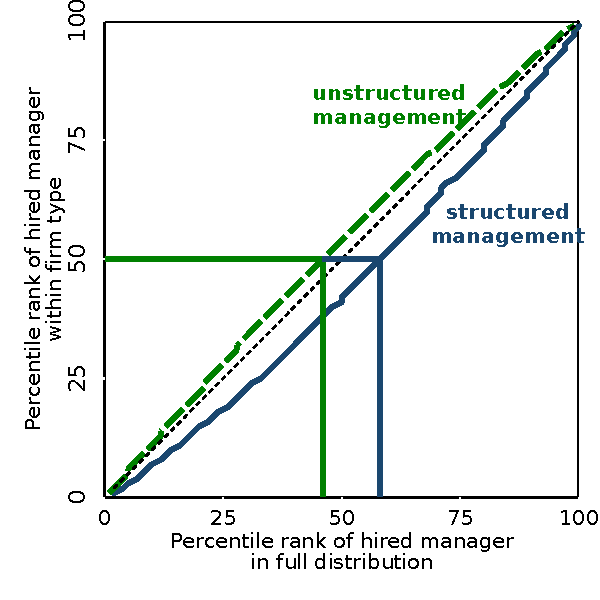
\includegraphics{./exhibits/fig_hiring_lorenz_mngr}
		\end{subfigure}
		\ \\
		\begin{subfigure}[b]{1\textwidth}
		  \centering
		   \caption{Production workers}
		  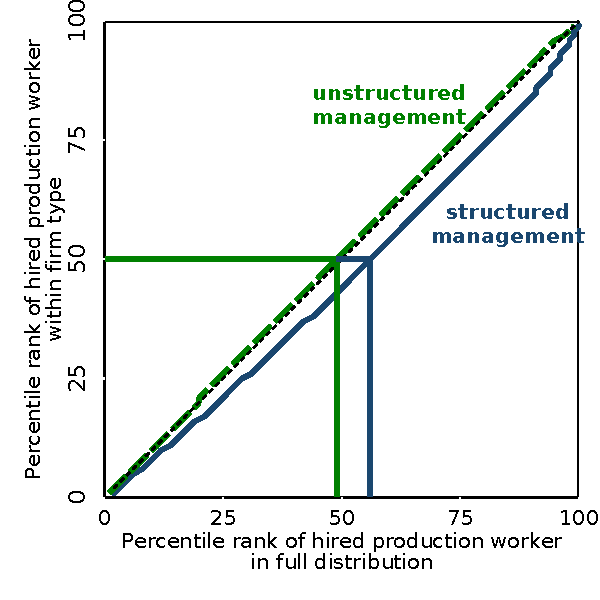
\includegraphics{./exhibits/fig_hiring_lorenz_labr}
		\end{subfigure}
		
	\end{figure}

% EXHIBIT: EMPLOYMENT SHARES BY WORKER QUALITY FOR STRUCTURED AD UNSTRUCTURED PROCESS FIRMS
\clearpage
	\begin{figure}[h]
		\centering
		\caption{Quality distribution of managers and production workers in continuing jobs}
		\label{fig:stayer_shares}
		\begin{subfigure}[b]{0.9\textwidth}
		  \centering
		  \caption{Managers}
		  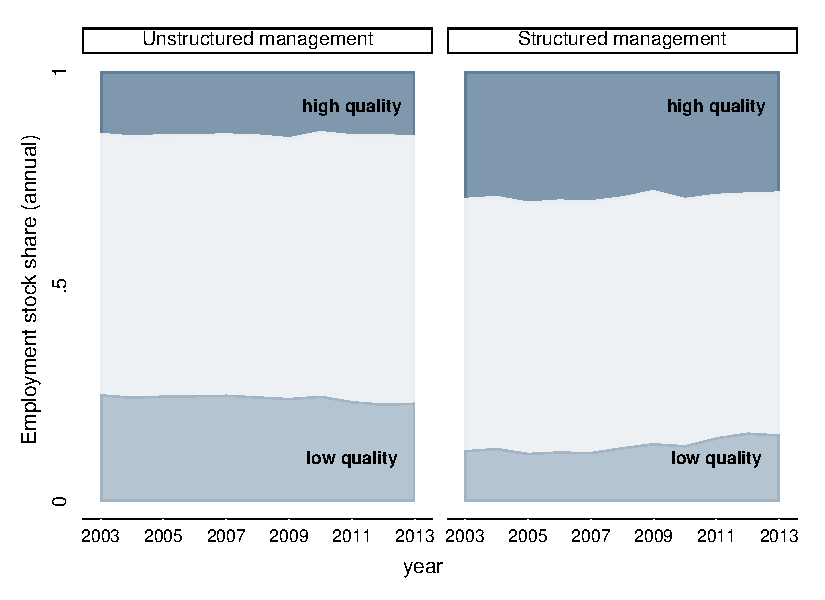
\includegraphics{./exhibits/fig_stayer_shares_mngr}\
		\end{subfigure}
		\ \\
		\begin{subfigure}[b]{0.9\textwidth}
		  \centering
		  \caption{Production workers}
		  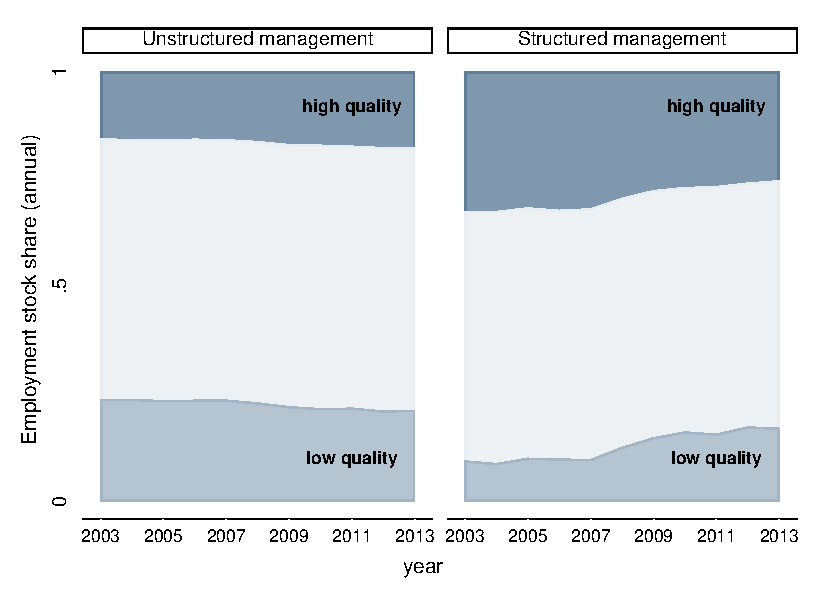
\includegraphics{./exhibits/fig_stayer_shares_labr}
		\end{subfigure}
	\end{figure}

% EXHIBIT: BIN SCATTERS OF FIRING RATES FOR MANAGERS AND PRODUCTION WORKERS
\clearpage
	\begin{figure}[ht]
		\centering
		\caption{Firing rates for managers and production workers by worker quality}
		\fbox{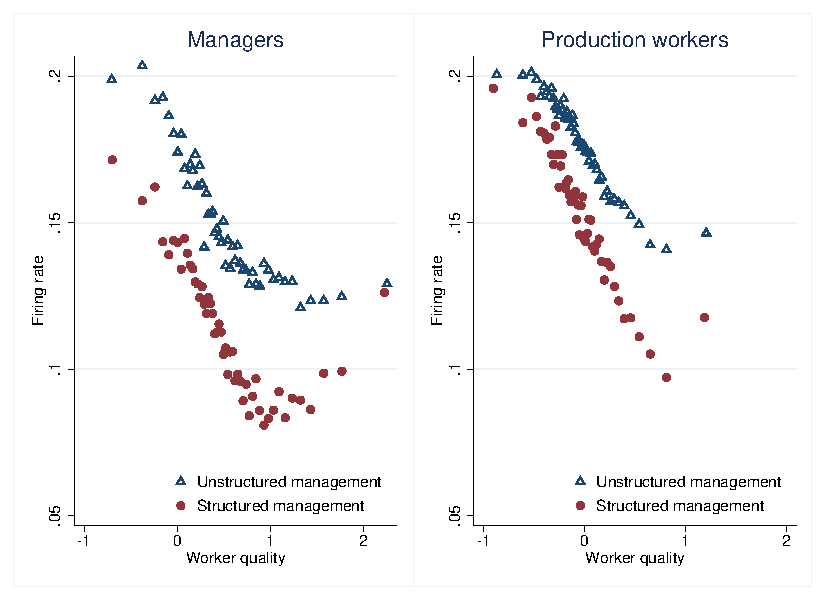
\includegraphics{./exhibits/fig_firing_binscatter}}
		\label{fig:firing_rate}
	\end{figure}
	
% EXHIBIT 5: TABLE 
\clearpage
\begin{landscape}
	\begin{table}
	\caption{Relationship between Worker and Management Quality} \label{tab:zpe_mgmt}
	\begin{center}
%	\scalebox{0.8}{
		\singlespace
		\small
		{
\begin{tabular}{l*{9}{c}}
\toprule
\textbf{Dependent variable:}  &\multicolumn{4}{c}{\textcolor{black}{z-(production worker quality)}}& & \multicolumn{4}{c}{\textcolor{black}{z-(manager quality)}} \\    \cline{2-5} \cline{7-10} 
				             &\multicolumn{1}{c}{(1)}&\multicolumn{1}{c}{(2)}&\multicolumn{1}{c}{(3)}&\multicolumn{1}{c}{(4)}&&\multicolumn{1}{c}{(5)}&\multicolumn{1}{c}{(6)}&\multicolumn{1}{c}{(7)}&\multicolumn{1}{c}{(8)}\\
                \midrule
 \textbf{Management indices} \\
z-people        &    0.100***&            &    0.098** &            &&    0.086***&            &    0.007   &            \\
                &  (0.036)   &            &  (0.042)   &            &&  (0.030)   &            &  (0.035)   &            \\
z-operations    &            &    0.074** &    0.004   &   -0.007   &&            &    0.143***&    0.137***&    0.130***\\
                &            &  (0.037)   &  (0.043)   &  (0.042)   &&            &  (0.033)   &  (0.040)   &  (0.040)   \\
                \\
\textbf{Individual practices} \\
z-talent mindset        &            &            &            &    0.091** &&            &            &            &    0.059*  \\
                &            &            &            &  (0.036)   &            &&            &            &  (0.031)   \\
z-performance culture        &            &            &            &    0.016   &&            &            &            &    0.008   \\
                &            &            &            &  (0.033)   &&            &            &            &  (0.032)   \\
z-talent capacity        &            &            &            &   -0.027   &&            &            &            &   -0.018   \\
                &            &            &            &  (0.033)   &&            &            &            &  (0.032)   \\
z-talent development        &            &            &            &    0.032   &&            &            &            &   -0.013   \\
                &            &            &            &  (0.041) &  &            &            &            &  (0.035)   \\
z-value proposition        &            &            &            &    0.016   &&            &            &            &   -0.015   \\
                &            &            &            &  (0.036)   &&            &            &            &  (0.037)   \\
z-retaining talent        &            &            &            &    0.017  & &            &            &            &   -0.009   \\
                &            &            &            &  (0.038)  & &            &            &            &  (0.033)   \\
Firm controls   &      Y   &      Y   &      Y   &      Y   &&      Y   &      Y   &      Y   &      Y   \\
Industry controls &      Y   &      Y   &      Y   &      Y   &&      Y   &      Y   &      Y   &      Y   \\
\midrule
\# Observations &\multicolumn{1}{c}{955}   &\multicolumn{1}{c}{955}   &\multicolumn{1}{c}{955}   &\multicolumn{1}{c}{955}   &&\multicolumn{1}{c}{955}  &\multicolumn{1}{c}{955}   &\multicolumn{1}{c}{955}   &\multicolumn{1}{c}{955}   \\
\# Firms        &      690   &      690   &      690   &      690   &&      690   &      690   &      690   &      690   \\
\(R^{2}\)       &    0.273   &    0.269   &    0.273   &    0.277   & &   0.353   &    0.360   &    0.360   &    0.362   \\
\bottomrule
\end{tabular}
}

%}
	\end{center}
\footnotesize{\textbf{Notes:} Results of linear regressions projecting plant-level averages of worker quality (estimated AKM worker effects) onto measures of management. 
In columns (1)--(4), the dependent variable is the average quality of production workers.
In columns (5)--(8), the dependent variable is the average quality of managers.
All models control for the log of employment, the year of observation (either 2008 or 2013), two-digit industry codes, the share of unionized workers, firm age, and whether the firm is multinational. 
In columns (1)--(3) and (5)--(7), the regressors of interest are the standardized measures of operations management and people management. In columns (4) and (8), the regressors of interest are the six subcomponents of the people-management measure. These measure the extent of structured management practices with respect to: (i) instilling a talent mindset; (ii) building a high-performance culture; (iii) making room for talent; (iv) developing talent; (v) creating a distinctive employee value proposition; (vi) retaining talent. For details of these different measures, see \citet{bloom_qje2007} and \citet{wms_jeea}.}
	\end{table}
\end{landscape}




























